%%%%%%%%%%%%%%%%%%%%%%%%%%%%%%%%%%%%%%%%%%%%%%%%%%%%%%%%%%%%%%%%%%%%%%%%%%%%%%%%
%2345678901234567890123456789012345678901234567890123456789012345678901234567890
%        1         2         3         4         5         6         7         8

%\documentclass[letterpaper, 10 pt, conference]{ieeeconf}  % Comment this line out
                                                          % if you need a4paper
\documentclass[a4paper, 11pt]{report}      % Use this line for a4
                                                          % paper

\usepackage[T1]{fontenc}
\usepackage{csquotes}
\usepackage{natbib}
\usepackage{graphicx}

%\usepackage{culmus}
%\usepackage{fontspec}
%\usepackage{polyglossia}
%\newfontfamily{\hebrewfont}{David CLM}


%\usepackage[english,hebrew]{babel}

%\selectlanguage{english}
\usepackage{fontspec}
\usepackage{appendix}

\bibliographystyle{abbrvnat}

\setcitestyle{authoryear,round}

\pagestyle{myheadings} 

\renewcommand{\thesection}{\arabic{section}}
%\DeclareUnicodeCharacter{}
% The following packages can be found on http:\\www.ctan.org
%\usepackage{graphics} % for pdf, bitmapped graphics files
%\usepackage{epsfig} % for postscript graphics files
%\usepackage{mathptmx} % assumes new font selection scheme installed
%\usepackage{mathptmx} % assumes new font selection scheme installed
%\usepackage{amsmath} % assumes amsmath package installed
%\usepackage{amssymb}  % assumes amsmath package installed

\begin{document}

\begin{titlepage} % Suppresses headers and footers on the title page
	
	{\centering % Centre everything on the title page
	% \rule{\textwidth}{1pt} % Thick horizontal rule
	
	% \vspace{2pt}\vspace{-\baselineskip} 
	% Whitespace between rules
	
	% \rule{\textwidth}{0.4pt} % Thin horizontal rule
		\vspace{0.05\textheight} % Whitespace between 
	
	%--------------------pastes randomly----------------------------
	%	Top rules
	%------------------------------------------------
	\huge{Department of Computer Science
	
	Bar-Ilan University
	
	\vspace{30pt}}
	\Large{
	M. Sc. Research Proposal - December 2020
	}
	\vspace{15pt}
	
	%\vspace{0.1\textheight} % Whitespace between the top rules and title
	
	%------------------------------------------------
	%	Title
	%------------------------------------------------
{\renewcommand{\baselinestretch}{1.8}\selectfont
    {\Huge \textsc{Investigation of team performance 
and physiological synchrony
in a musical coordination taks}} % Title line 
\par}

	
	\vspace{0.025\textheight} % Whitespace between the title and short horizontal rule
	
	\rule{0.3\textwidth}{0.4pt} % Short horizontal rule under the title 
    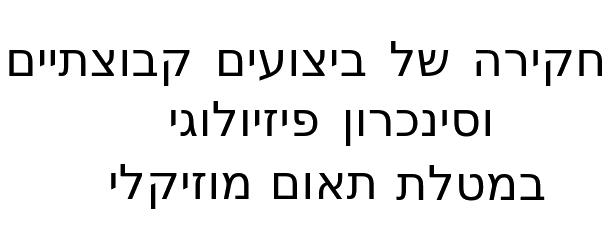
\includegraphics[scale=0.7]{hebrew_title1s.png}
%	\vspace{0.1\textheight}
%	\par% Whitespace between 
%	\vspace{0.1\textheight} % Whitespace between the thin horizontal rule and the author name
%\selectlanguage{English}
	
	\vspace{0.01\textheight} % Whitespace between 
	\rule{0.3\textwidth}{0.4pt} % Short horizontal rule under the title
	
	\vspace{10pt} % Whitespace between the thin horizontal rule and the author name
	
	%------------------------------------------------
	%	Author
	%------------------------------------------------
	
	{\Large \bf Shahar Siegman}\par
	
	}% Author name
	
	
	\vspace{0.05\textheight} % Whitespace between the 

	{\Large  Advisors: \par 
	\bf Ronny Bartsch \par}
	{\large Bar Ilan Physics Dept.\par} 
	{\Large \bf Ilanit Gordon \par} 
	{\large The Gonda Multidisciplinary Brain Research Center}  % Author name
	
	%------------------------------------------------
	%	Publisher
	%------------------------------------------------
	
	

	%\vfill % Whitespace under the publisher text
	
	%------------------------------------------------
	%	Bottom rules
	%------------------------------------------------
	
	%\rule{\textwidth}{0.4pt} % Thin horizontal rule
	
	%\vspace{2pt}\vspace{-\baselineskip} % Whitespace between rules
	
	%\rule{\textwidth}{1pt} % Thick horizontal rule
	
\end{titlepage}

%\selectlanguage{English}


%%%%%%%%%%%%%%%%%%%%%%%%%%%%%%%%%%%%%%%%%%%%%%%%%%%%%%%%%%%%%%%%%%%%%%%%%%%%%%%%
{\renewcommand{\baselinestretch}{1.3}\selectfont
\tableofcontents
}

\pagebreak

\chapter{Background}
\section{Synchrony in physiological signals}
Physiological synchrony (PS) occurs when the development in time of the measured physiological states of two or more individuals, align in a way that implies a common causal factor and matched phase. Of particular interest are measures regulated by the autonomous nervous system (ANS). Synchrony in such signals has been shown to occur in varied social settings, including among family members, between friends, in people interacting for the first time, and even in the womb and while co-sleeping (\cite{palumbo2017interpersonal}; \cite{jar202physiological}; \cite{ivanov2009maternal}; \cite{yoon2019human}). The current study focuses on synchrony in  inter-beat intervals, a continuous-time measure extracted from ECG readings. 

Despite the wide success in demonstrating PS in ANS-related signals,  there remain significant theoretical gaps in understanding the details of the dynamics as well as the underlying mechanisms  \citep{jar202physiological}. 
One proposed mechanism for how PS forms, is through the common psychological experience, leading to synchronized patterns of autonomous nervous system (ANS) activity, which in turn influence the physiological signals in a similar fashion \citep{palumbo2017interpersonal}. A more direct mechanism was suggested by \citet{behrens2020physiological}, who 
demonstrated that visual cues, such as subtle changes in facial expression, are constructive in forming synchrony. 

\section{Physiological synchrony in the study of team performance}
Team performance is a long-established research topic in social sciences. Team performance has been linked to better individual (subjective) experiences during the interaction \citep{lodahl1961psychometric}, and also to group cohesiveness -- the desire of team members to be part of the group \citep{cartwright1968nature}. Still, despite decades of research, our understanding of this field is fragmented, with limited success in generalizing the proposed theoretical models and in recreating findings across setups. As  \citet{beal2003cohesion} noted, this state of affairs is partially attributable to the large variation in experimental and observational setups, as well as in the ensuing analysis approaches. Modeling team performance remains a matter of active research, see for example \citet{collins2019explorations}.

For well over a decade now, researchers have been harnessing PS for the study of group performance. An eloquent herald of this trend is \citet{akinola2010measuring}, which suggested that physiological measures be incorporated into the (metaphoric) toolbox of the organizational researcher as a way to \enquote{deepen theoretical insights and enrich our understanding of human behavior in organizations}. More recently,  \citet{chikersal2017deep} have demonstrated a correlation between shared arousal, as measured by electrodermal activity (EDA), and group satisfaction. Another interesting recent example is \citet{danyluck2018intergroup}, which have taken a different approach to incorporating physiological measurements in the study of group performance. Casting physiological synchrony as the outcome, they examined which of the different priming levels induces a higher level of PS. Check out \citet{jar202physiological} for a list of several additional works involving PS and group performance.

\section{Musical coordination tasks}
In the current experiment, musical coordination was the desired outcome. Groups of three participants engaged in two successive sessions in which they were instructed to play musical drums together. Physiological signals were measured before, during, and after each session\footnotemark. 
\footnotetext{for more details on the current experiment, see Appendix A below, or refer to \cite{gordon2020physio}.} 
This setup allows us to test for emerging patterns of coordination within the performing group, and how they are portended or accompanied by patterns of physiological synchrony.

Analysis of synchrony patterns in group playing tasks was also performed in  \cite{abp2017symmetry} and \cite{shahal2020synchronization}. These studies focus on the emergence and stability of patterns of synchronicity in playing. We believe our work is unique in examining musical coordination and PS together.

\chapter{Proposed contributions}

\section{Prior results for the drumming experiment}

In \cite{gordon2020physio}, cross correlation function analysis yielded maximal pairwise correlations between IBI signals from the three participants of each group, taking one pair at a time. Then, the three pairwise coefficients  were averaged to yield a group physiological synchrony index. This index was shown to predict about 15\% of the variability in \emph{group cohesion}, a psychological index calculated based on responses to a questionnaire filled out by the participants between the two playing sessions. 

Additionally, drumming coordination during the second drumming session was scored based on number of co-occurring drum beats. The group's IBI synchrony was found to predict this cooridnation index, to a certain extent.   

\section{New contributions in this study}

In this study, we build on the above analysis, extending it in several respects.


First, we suggest that a more comprehensive description of the synchrony in the heart-rate inter-beat-interval (IBI) signal is obtained when the IBI is broken down into a high-frequency signal and a low-frequency signal. We intend to demonstrate that using these two components as two separate causal factors, improves the predictive model.


Second, we streamline the process of extracting the heart rate variability (HRV) by calculating a \enquote{moving RMS} of the high-frequency component. We demonstrate that this HRV time series is generally uncorrelated with the high-frequency signal from which it was derived, and is therefore a third aspect of the IBI signal, in which synchrony among individuals can be checked. We verify the existence of correlations of HRV within the groups.  

Third, we elaborate the quantitative analysis of the drumming coordination. We apply \emph{discrete relative phase analysis} \citep{abp2017symmetry} between pairs of drumming signals, followed by entropy calculation on the resulting distribution, to extract an index for beat-to-beat drumming coordination. We also look at correlations in beat pacing during the session. These constitute enhancements to the single coordination index in the previous work.

Fourth, we embed the heart-rate IBI signals in 2D space in order to characterize synchrony in triads. We use \emph{angular distances} as the distance metric between signals, allow us to visualize each triad as a triangle. The scales and shapes of the triangles, correspond to first- and second-order statistics of the group's synchrony. We intend to demonstrate that, on top of the appeal of this model due to its clear intuition, the use of the second-order statistic helps explain the target variables, namely the group cohesion and drumming coordination.

Fifth, we use the richer descriptions of both the heart-rate synchorny and the drumming coordination  to establish a more nuanced quantitative relationship between the physiological and the sensorimotor aspects of the interaction, and to discover thus-far overlooked links between the different variables.  

\section{Contributions based on methods from computer science}
We'd like to point to the original contributions that are, or likely will, involve methods developed in the domains of computer science and statistical machine learning.

The mathematical notion of a distance metric is often applied in machine learning in order to find similar samples and to embed a high-dimensional data point in a low-dimensional space. Here, it will help in summarizing the relationships among the three signals.

Shannon entropy will be employed in order to derive a distance measure from the drumming's relative phase charts.

Finally, our research involves characterizing relationships and finding interesting connections among several variables: synchrony indices in different bands and during different sessions; drumming performance indices in two separate drumming sessions; psychological traits and reactions to the group interaction. This is essentially a task of knowledge discovery in databases (KDD), where a large array of supervised and unsupervised machine learning methods may be applied. Admittedly, we will have to be very prudent when choosing our methods due to the small number of records at our disposal. Some methods that we consider apt given the volume of data are classification and regression trees (CART), clustering analysis, and latent-variable modeling using the expectation-maximization (EM) algorithm.




\chapter{Preliminary results}

\section{RMS signal synchrony}

Here's a plot illustrating how RMS signals is extracted from the high-frequency component of the IBI signal:


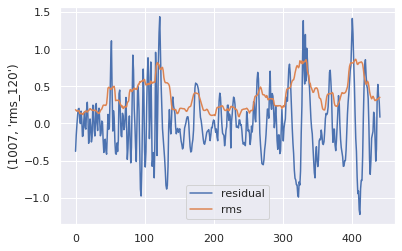
\includegraphics[scale=0.5]{residual_rms_example.png}

and here, by using the technique of surrogate analysis (matching signals from different groups), we demonstrate the synchrony in rms:

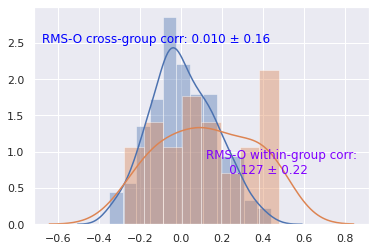
\includegraphics[scale=0.5]{rmso_within_and_cross.png}

\section {2D space embeddings of signals}

The below image shows the relationships between the IBI signals in the first drumming session, after embedding in 2D space using angular distance as the distance metric.

\vspace{1cm}

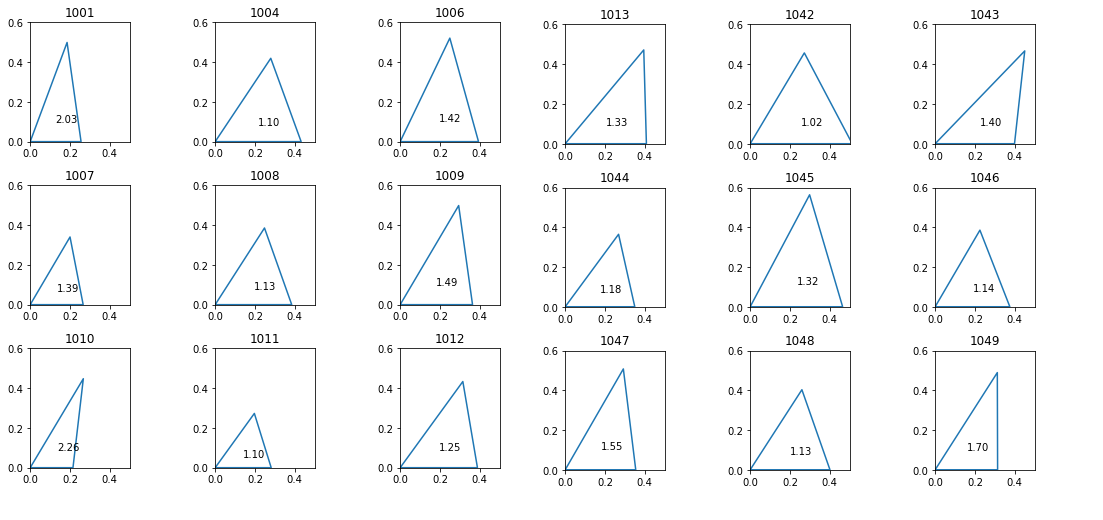
\includegraphics[scale=0.35]{triangles_coupling_modes_landscape.png}


\appendix
\chapter{Experiment Details}
\section{Technical background on heart rate}
The signal to be analyzed in the current work is the heart rate, or IBI interval. 
The heart rate is measured by analyzing the electric potential between electrodes placed on the subject's torso. The RR-interval, a name derived from the "R" peak in the ECG, is the interval between successive beats, in other words, the instantaneous reciprocal of the heart rate. The variation of heart rate over time in healthy individuals is controlled by several different pathways in the autonomous nervous system. In many different settings, persons in direct social contact (i.e. in physical proximity and exchanging social cues) have been observed to have some level of synchrony in their heart rates over the course of an experiment, which is understood as an affirmation of the fact that the regulatory states of the two individuals are both affected by (or respond to) the cues exchanged during their social interaction \citep{palumbo2017interpersonal}.
The RR-interval is also known as the inter-beat interval, or IBI.

\section{Experiment itinerary and details of data recorded}
A brief description of the experiment on which this work focuses follows. The experiment as described below was repeated 50 times, with different teams of three members each. For more details, see \cite{gordon2020physio}.
\begin{itemize}
    \item Before arriving, each participant had to fill in and submit a personality questionnaire which focuses on social affinity.
    \item Just before the interaction started, the participants filled another questionnaire, regarding their current mood, sleep, and caffeine intake.

    \item Each team's interaction was subdivided into 4 sessions. The sessions were recorded (video, audio), and electrodes were used to collect continuous ECG readings from the participants. 
    \begin{itemize}
        \item In the first session, team members were simply asked to relax. This is the first of two \emph{baseline} sessions.
        \item In the second session, team members were instructed to follow a pre-recorded tempo. Each participant played on his or her own electronic drum pad, allowing us to record the beats of each player. This session lasted 4 minutes. Half the teams were randomly selected for one type of tempo, and the other half followed a different tempo.
        \item At this point, the participants filled in their responses to questions regarding both perceived drumming synchrony, and affect.
        \item Next, each team played the drums again, this time without any background tempo (\emph{freestyle} session).
        \item Following the freestyle sessions, an additional round of questions regarding affect was administered. 
        \item In the final session, the team members again were in the same room without performing any task. This is the second baseline session.
    \end{itemize}
\end{itemize}
Note: Participants were pre-screened for musical  background. Respondents with significant musical experience were not admitted.




\bibliography{ref}
\end{document}

